\chapter{States of the World and Asset Pricing}

Assets give a \textit{payoff} $x_{t+1}$. In our focus on stocks, 
$x_{t+1} = p_{t+1} + d_{t+1}$, where $p_{t+1}$ is the 
price of the stock at time $t+1$ and $d_{t+1}$ 
is the dividend paid at time $t+1$.
$x_{t+1}$ is a random variable, like a coin-flip - we don't 
know at $t$ what it will be at $t+1$. But we can assign 
probabilities to the possible outcomes of $x_{t+1}$.
We can think of the \textit{randomness} of $x_{t+1}$ as being
due to the randomness of the \textit{state of the world} at $t+1$.
$x_{t+1}$ takes on different values in 
different \textit{states of the world}.
We have:

\begin{equation}
    E(x_{t+1}) = \sum_s \pi(s) x(s)
\end{equation}

where $E(x_{t+1})$ is the expected value of $x_{t+1}$,
$\pi(s)$ is the probability of state $s$, and $x(s)$ is the
value of $x_{t+1}$ in state $s$.

The question we are trying to answer here is: what is the price 
or value $p_t$ of the payoff $x_{t+1}$ at time $t$?

\begin{figure}[htbp]
    \centering
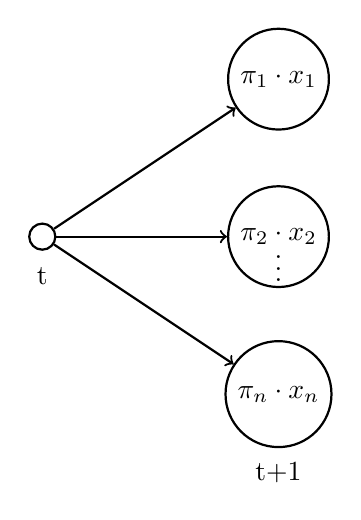
\begin{tikzpicture}[->, thick, auto, node distance=3cm]
    % Nodes at t
    \node[circle, draw] (t) at (0, 0) {};
    
    % Nodes at t+1
    \node[circle, draw] (t1s1) at (3, 2) {\(\pi_1 \cdot x_1\)};
    \node[circle, draw] (t1s2) at (3, 0) {\(\pi_2 \cdot x_2\)};
    \node[circle, draw] (t1sn) at (3, -2) {\(\pi_n \cdot x_n\)};

    % Edges
    \draw (t) -- (t1s1);
    \draw (t) -- (t1s2);
    \draw (t) -- (t1sn);
    
    % Labels for time
    \node at (0, -0.5) {t};
    \node at (3, -3) {t+1};
    
    % Dots for multiple nodes
    \node at (3, -0.3) {\(\vdots\)};
\end{tikzpicture}
    \caption{States of the world at time \(t+1\)}
    \label{fig:states_of_the_world}
\end{figure}

\section{Utility and Asset Pricing}


\begin{tcolorbox}[colback=white, colframe=black, title=Example X]
    xxx
\end{tcolorbox}

\section{Risk Valuation}

To apply what we have learned so far to risk valuation, we can start
from the definition of the covariance:

\begin{equation}
    \text{Cov}(m, x) = E(mx) - E(m)E(x)
\end{equation}

Thus,

\begin{equation}
    p = E(mx) = \text{Cov}(m, x) + E(m)E(x)
\end{equation}

\begin{equation}
    p = \frac{1}{R^f} E(x) + \text{Cov}(m, x)
\end{equation}

with the approximation

\begin{equation}
    m_{t+1} \approx 1 - \delta - \gamma \Delta c_{t+1}
\end{equation}

we have

\begin{equation}
p^i_t \approx \frac{1}{R^f} E(x^i_{t+1}) + \text{Cov}(x^i_{t+1}, \Delta c_{t+1})
\end{equation}

That is, the price is lower if the asset do well 
when consumption is low, and vice versa. Prices are higher 
for assets that provide insurance against consumption risks.
Prices are low for assets that, if you buy them, make your consumption
more risky. 

In risk valuation, the covariance term really matters. 
The same $m$ and the same $x$ can have different prices depending on the covariance between
$m$ and $x$. 

\begin{tcolorbox}[colback=white, colframe=black, title=Example 1]
Suppose there are two states $u$ and $d$ tomorrow, with probability
$1/2$ each. In state $u$, consumption is high, and in state $d$,
consumption is low.

\begin{equation}
    p_t = E(m, x) = \frac{1}{2} m_u x_u + \frac{1}{2} m_d x_d
\end{equation}


Suppose $x$ pays off well in good times if $x_u = 2$ and 
$x_d = 1$. Suppose also that $m_u = 0.5$ and $m_d = 1$. 
Then,

\begin{equation}
    p_t = \frac{1}{2} \times 0.5 \times 2 + \frac{1}{2} \times 1 \times 1 = 1
\end{equation}

Now suppose we keep the same volatility but $x$ pays off well 
in bad times and badly in good times, with $x_u = 1$ and $x_d = 2$.

Then,

\begin{equation}
    p_t = \frac{1}{2} \times 0.5 \times 1 + \frac{1}{2} \times 1 \times 2 = 1.25
\end{equation}

The payoff is worth more in the second case because it pays off
more in bad times, that is when $m$ is high (hungry) rather 
than $m$ is low (full). 
$m$ acts like a price: it says that payoffs 
delivered in the bad state of nature $d$ worth more than 
payoffs delivered in the good state of nature $u$.

\end{tcolorbox}